% vim:fdl=0:wrap
\documentclass[a4paper, 11pt]{article}           %{{{1
% basic packages                                  {{{2
\usepackage[T1]{fontenc}
\usepackage[scaled=0.975]{helvet}
\usepackage[utf8]{inputenc}
\usepackage{amsmath}
\usepackage{lastpage}
\usepackage{graphicx}
\usepackage{amsfonts}
\usepackage{variations}
\usepackage{pgf,tikz}           % dessin
\usepackage{mathrsfs}
\usetikzlibrary{arrows}
\usepackage{pgfkeys}        % fenetrage des plot TikZ
\usepackage{yhmath}         % arc au dessus des lettres
\usepackage{calc}           % calcul de longueur
\usepackage{multicol}
\usepackage{enumitem}
\usepackage{tcolorbox}                                                          % encadrement texte
% ==== PROGRAMMATION
\usepackage{xcolor}                                                             %
\usepackage{listings}                                                           %
% listings                                        {{{3
\definecolor{mygreen}{rgb}{0,0.6,0}
\definecolor{mygray}{rgb}{0.5,0.5,0.5}
\definecolor{mymauve}{rgb}{0.58,0,0.82}
\definecolor{deepblue}{rgb}{0,0,0.5}
\definecolor{deepred}{rgb}{0.6,0,0}
\definecolor{deepgreen}{rgb}{0,0.5,0}
\lstset{%
%       backgroundcolor=\color{white},   % choose the background color; you must add \usepackage{color} or \usepackage{xcolor}; should come as last argument
        basicstyle=\tiny,          % the size of the fonts that are used for the code
%       breakatwhitespace=false,         % sets if automatic breaks should only happen at whitespace
%       breaklines=true,                 % sets automatic line breaking
%       captionpos=b,                    % sets the caption-position to bottom
        commentstyle=\color{mygreen},    % comment style
%       deletekeywords={type},           % if you want to delete keywords from the given language
%       emph={},                         % Custom highlighting
%       emphstyle=\ttb\color{deepred}    % Custom highlighting style
%       escapeinside={\%*}{*)},          % if you want to add LaTeX within your code
%       extendedchars=true,              % lets you use non-ASCII characters; for 8-bits encodings only, does not work with UTF-8
        frame=shadowbox,                 % adds a frame around the code {single, shadowbox}
%       keepspaces=true,                 % keeps spaces in text, useful for keeping indentation of code (possibly needs columns=flexible)
        keywordstyle=\color{blue},       % keyword style
	language=C,                      % the language of the code {Python, C}
%       morekeywords={*,...},            % if you want to add more keywords to the set
        numbers=left,                    % numbers = (none, left, right)
%       numbersep=5pt,                   % how far the line-numbers are from the code
%       numberstyle=\tiny\color{mygray}, % the style that is used for the line-numbers
%       otherkeywords={self},            % Add keywords here
%       rulecolor=\color{black},         % if not set, the frame-color may be changed on line-breaks within not-black text (e.g. comments (green here))
	rulesepcolor=\color{gray}        % shadowbox color
%       showspaces=false,                % show spaces everywhere adding particular underscores; it overrides 'showstringspaces'
%       showstringspaces=false,          % underline spaces within strings only
%       showtabs=false,                  % show tabs within strings adding particular underscores
%       stepnumber=1,                    % the step between two line-numbers. If it's 1, each line will be numbered
%       stringstyle=\color{mymauve},     % string literal style
%       tabsize=4,                       % sets default tabsize to 2 spaces
%       title=\lstname                   % show the filename of files included with \lstinputlisting; also try caption instead of title
}
%}}}
%}}}

% mise en page                                    {{{2
\addtolength{\voffset}{-1.8cm}
\addtolength{\textheight}{4cm}
\addtolength{\hoffset}{-2.5cm}
\addtolength{\textwidth}{4cm}
\addtolength{\headsep}{-0.5cm}
\usepackage{fancyhdr}
\setlength{\headheight}{14.00pt}
\pagestyle{fancy} % Numérotation des pages
\renewcommand\headrulewidth{1pt}
\renewcommand\footrulewidth{1pt}
\fancyhead[L]{BP SN}
\fancyhead[C]{arduino}
\fancyhead[R]{RFID}
\fancyfoot[L]{v 1.5 -- JB}
\fancyfoot[C]{gestion de l'habitat | gestion de l'accès }
\fancyfoot[R]{\thepage/\pageref{LastPage}}
%\lhead{3E}%haut de page gauche
%}}}

% Compteurs:                                     {{{2
\addtocounter{page}{0}
\newcounter{Q}
\newcounter{exoNB}
%}}}

% newcommand                                     {{{2
\newcommand{\objectif}[1]{\textsc{\huge \textbf{Objectif :}\\[2mm] #1} }
\newcommand{\partie}[1]{\textsc{\LARGE #1} }

\newcommand{\question}{\stepcounter{Q} $\boxed{\arabic{Q}}$ }
\newcommand{\reponse}{
\par\nobreak
\noindent\rule{0pt}{1.5\baselineskip}% Provides a larger gap between the preceding paragraph and the dots
{\noindent\makebox[\linewidth]{\dotfill}\endgraf}% ... dotted lines ...
% \bigskip% Gap between dots and next paragraph
}


\newcommand{\ligne}{\underline{\hspace{ \textwidth}} }
\newcommand{\exo}[1]{\stepcounter{exoNB}\textsc{\Large Exercice \arabic{exoNB} -- #1} }
\newcommand{\EXO}[2]{\stepcounter{exoNB}\textsc{\Large Exercice \arabic{exoNB} -- #1} \hfill \textbf{#2 points}}
\newcommand{\pb}[1] {\stepcounter{exoNB}\textsc{\Large Problème \arabic{exoNB} -- #1} }
\newcommand{\PB}[2] {\stepcounter{exoNB}\textsc{\Large Problème \arabic{exoNB} -- #1} \hfill \textbf{#2 points}}
%}}}

% Longueur:                                      {{{2
\newlength{\longueurA}
\newlength{\longueurB}
\setlength{\parindent}{0pt}
\setlength{\parskip}{2pt}
\renewcommand{\baselinestretch}{1}
%}}}

% Divers                                          {{{2
% listings                                        {{{3
%\definecolor{mygreen}{rgb}{0,0.6,0}
%\definecolor{mygray}{rgb}{0.5,0.5,0.5}
%\definecolor{mymauve}{rgb}{0.58,0,0.82}
%\definecolor{deepblue}{rgb}{0,0,0.5}
%\definecolor{deepred}{rgb}{0.6,0,0}
%\definecolor{deepgreen}{rgb}{0,0.5,0}
%\lstset{%
%        backgroundcolor=\color{white},   % choose the background color; you must add \usepackage{color} or \usepackage{xcolor}; should come as last argument
%        basicstyle=\footnotesize,        % the size of the fonts that are used for the code
%        breakatwhitespace=false,         % sets if automatic breaks should only happen at whitespace
%        breaklines=true,                 % sets automatic line breaking
%        captionpos=b,                    % sets the caption-position to bottom
%        commentstyle=\color{mygreen},    % comment style
%        deletekeywords={...},            % if you want to delete keywords from the given language
%        escapeinside={\%*}{*)},          % if you want to add LaTeX within your code
%        extendedchars=true,              % lets you use non-ASCII characters; for 8-bits encodings only, does not work with UTF-8
%        frame=single,                    % adds a frame around the code
%        keepspaces=true,                 % keeps spaces in text, useful for keeping indentation of code (possibly needs columns=flexible)
%        keywordstyle=\color{blue},       % keyword style
%        morekeywords={*,...},            % if you want to add more keywords to the set
%        numbers=left,                    % where to put the line-numbers; possible values are (none, left, right)
%        numbersep=5pt,                   % how far the line-numbers are from the code
%        numberstyle=\tiny\color{mygray}, % the style that is used for the line-numbers
%        rulecolor=\color{black},         % if not set, the frame-color may be changed on line-breaks within not-black text (e.g. comments (green here))
%        showspaces=false,                % show spaces everywhere adding particular underscores; it overrides 'showstringspaces'
%        showstringspaces=false,          % underline spaces within strings only
%        showtabs=false,                  % show tabs within strings adding particular underscores
%        stepnumber=2,                    % the step between two line-numbers. If it's 1, each line will be numbered
%        stringstyle=\color{mymauve},     % string literal style
%        tabsize=4,                       % sets default tabsize to 2 spaces
%        title=\lstname                   % show the filename of files included with \lstinputlisting; also try caption instead of title
%}
%\lstset{%
%        language=Python,                 % the language of the code
%        otherkeywords={self},            % Add keywords here
%        deletekeywords={type},           % if you want to delete keywords from the given language
%        emph={},                         % Custom highlighting
%        emphstyle=\ttb\color{deepred}    % Custom highlighting style
%}
%}}}

% PRL style line                                 {{{3
\newlength{\diamondrulelength}
\setlength{\diamondrulelength}{0.6\textwidth}
\newlength{\diamondrulethickness}
\setlength{\diamondrulethickness}{2pt}
\newcommand{\diamondrule}{\begin{center}\tikz{\fill[black] (0.5\diamondrulelength,0) -- (0,0.5\diamondrulethickness) -- (-0.5\diamondrulelength,0) -- (0,-0.5\diamondrulethickness) -- cycle;}\end{center}}
%}}}

% fixed with tabular                             {{{3
\usepackage{array}
\newcolumntype{L}[1]{>{\raggedright\let\newline\\\arraybackslash\hspace{0pt}}m{#1}}
\newcolumntype{C}[1]{>{\centering\let\newline\\\arraybackslash\hspace{0pt}}m{#1}}
\newcolumntype{R}[1]{>{\raggedleft\let\newline\\\arraybackslash\hspace{0pt}}m{#1}}
%}}}

%}}}
%}}}

\begin{document}
\sffamily
\hfill Nom : {\noindent\makebox[5cm]{\dotfill}\endgraf}
\objectif{Support d'identification, lecteurs, unités de traitement, gestion de communication}\\


L'utilisation MF RC522 met en oeuvre la modulation et la démodulation à 13.56MHz. Elles sont complètement intégrées avec toutes sortes de méthodes de communication sans contact et de protocoles. La partie numérique gère les cadres ISO14443A et la détection d'erreur, l'algorithme de cryptage Quick CRYPTO1, et le terme de vérification série MIFARE.

Le module MFRC522 prend en charge le protocole  de communications sans contact à haute vitesse MIFARE, avec des taux de transfert de données bidirectionnels jusqu'à 424 kbit/s. Le module MF522 utilise un composant d'origine Philips MFRC522 lecteur de carte de circuit. Il est facile à utiliser, faible coût, adapté au développement de l'équipement. Il prend en compte la nécessité de conception de terminal RF / utilisateurs de production. Ce module peut être directement chargé dans la multitude de forme de lecteur. Le module utilise une tension de 3.3V. Avec seulement quelques lignes simples à travers l'interface SPI, tout utilisateur connecte directement le CPU au module de communication, et peut de plus garantir un travail stable et fiable, distance du lecteur.\\

\partie{Materiel} \\                      %{{{1
\begin{minipage}{.4\textwidth} %
Current:13-26mA / DC 3.3V \\
Idle Current:10-13mA / DC 3.3V \\
Sleep current: <80uA \\
Peak current: <30mA \\
Operating Frequency: 13.56MHz \\
Environmental Operating temperature: -20 to 80 degrees Celsius \\
Environment Storage temperature: -40 to 85 degrees Celsius \\
Relative Humidity: 5\% -95\% \\
\end{minipage}
\begin{minipage}{0.6\textwidth} %
\begin{center}
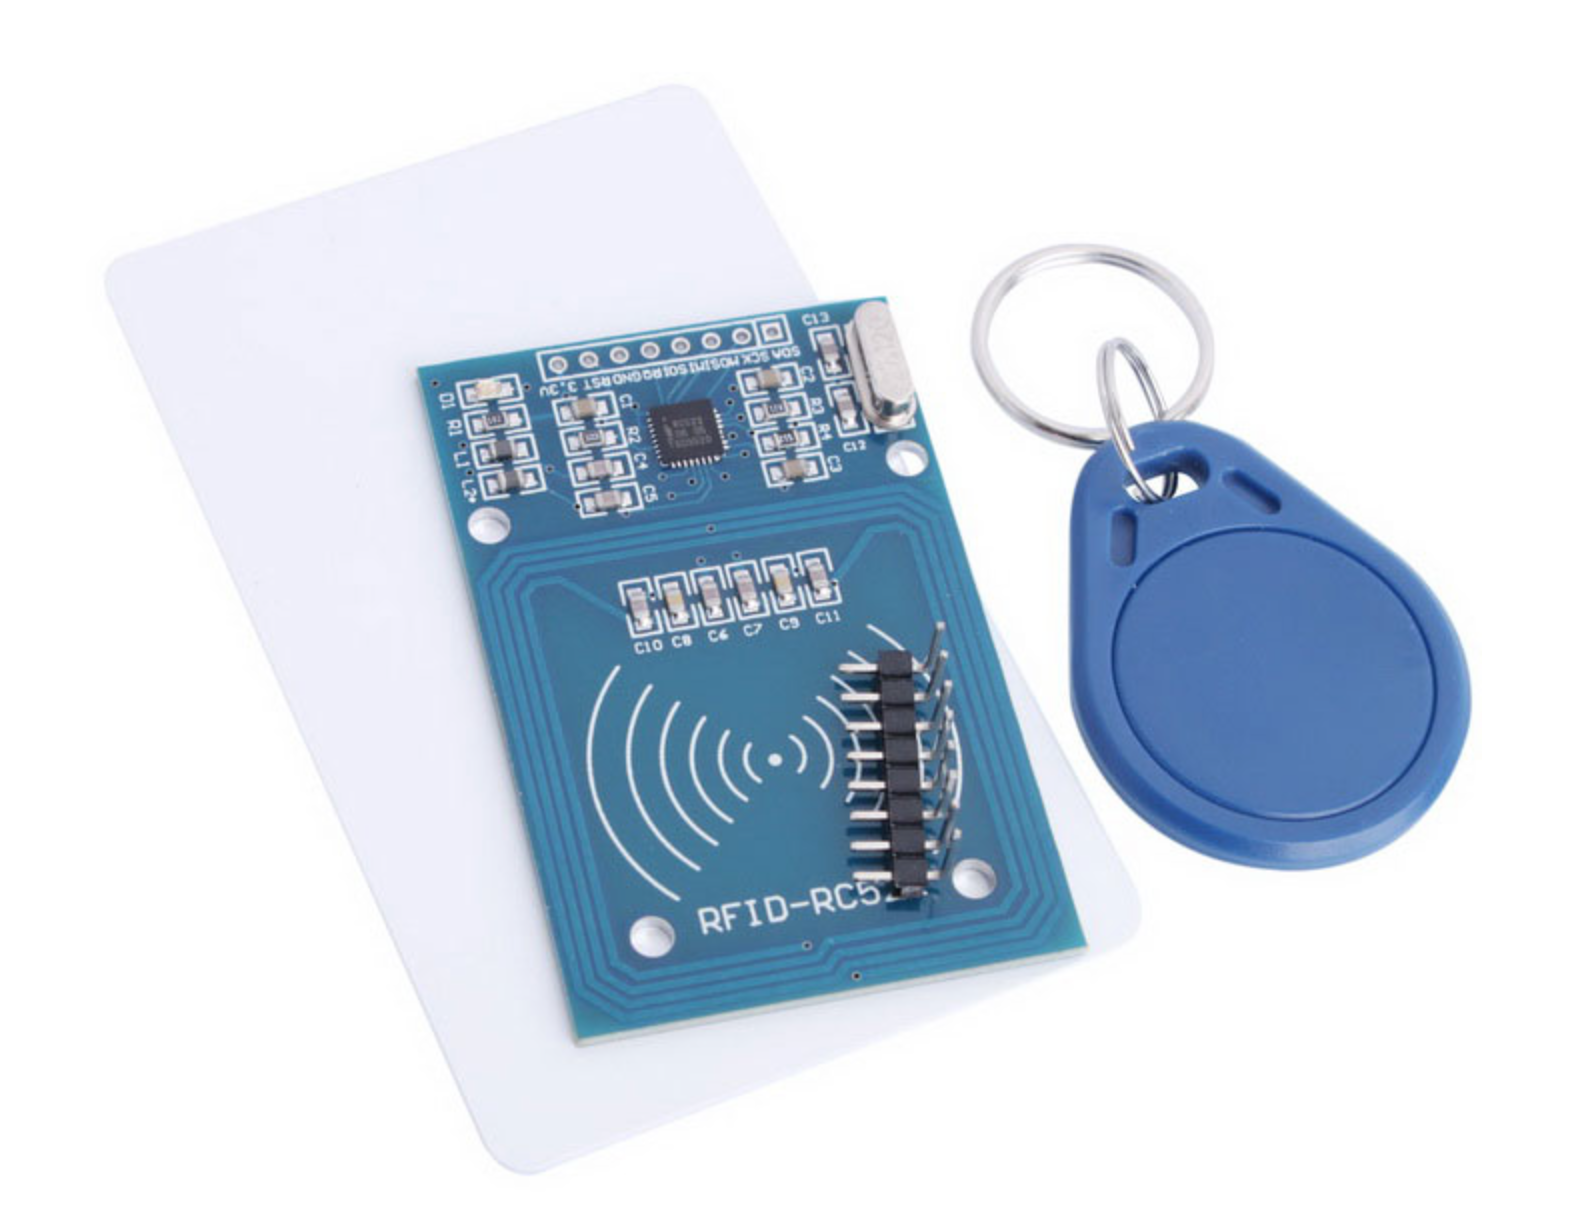
\includegraphics[width=0.8\textwidth]{RC522}\\
tag RFID et son lecteurs
\end{center}
\end{minipage}

%}}}

\partie{Lire le tag}\\ %{{{1

\question Est-ce que le dispositif comporte une source d'énergie comme une pile ?
\reponse

\question Quelle est alors l'origine de l'énergie faisant marcher les composants sur le tag ?
\reponse

\question A quel composant d'électronique de puissance vous fait penser cette gestion de l'énergie ?
\reponse

\question Une fois que votre montage marchera, tester la distance maximale à laquelle la communication fonctionne ?
\reponse

\question Installer la librairie du RC522 (voir figure \ref{FigBibliotheque} ) et la tester.
\begin{figure}[p]
\begin{center}
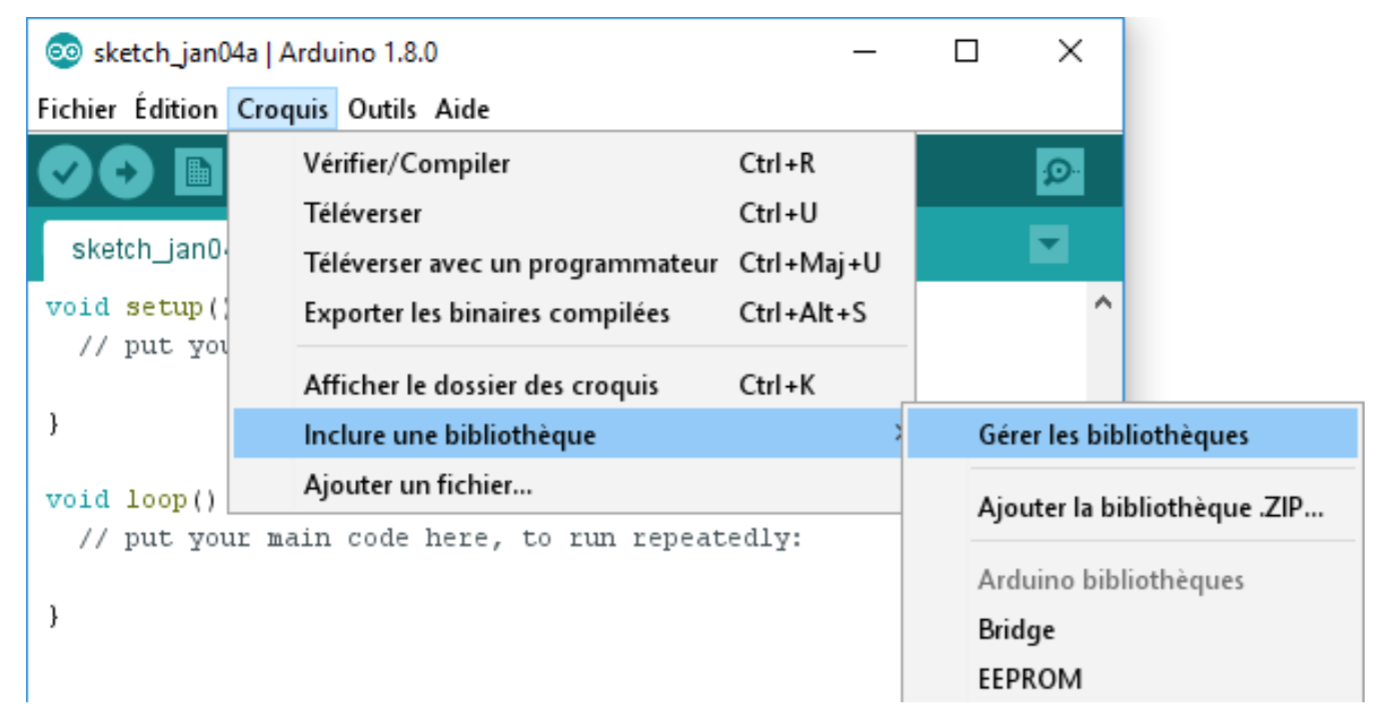
\includegraphics[width=\textwidth]{bibliotheque_inclure}
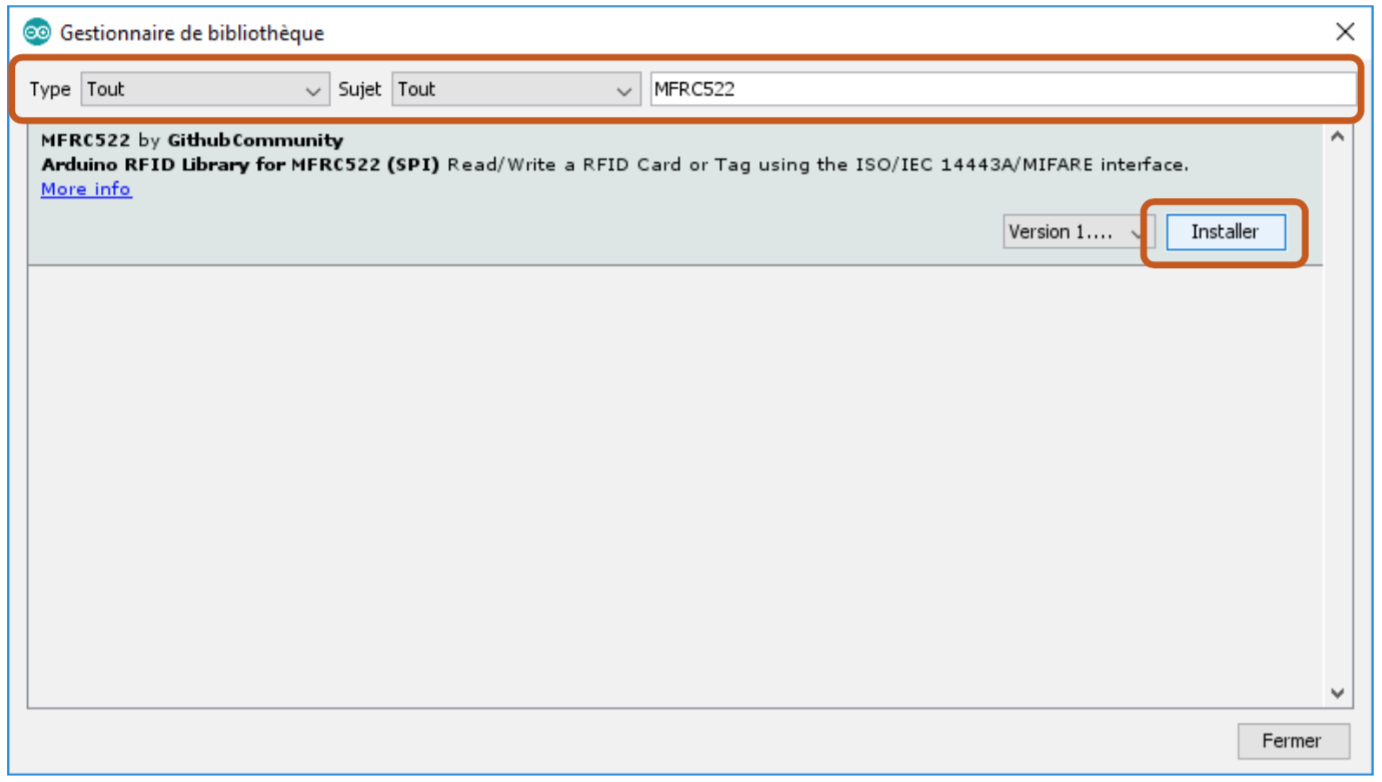
\includegraphics[width=\textwidth]{bibliotheque_installer}
\caption{installation de la librairie SPI pour la carte RFID}
\label{FigBibliotheque}
\end{center}
\end{figure}

\question Branchement\\

\begin{figure}[!h]
\begin{center}
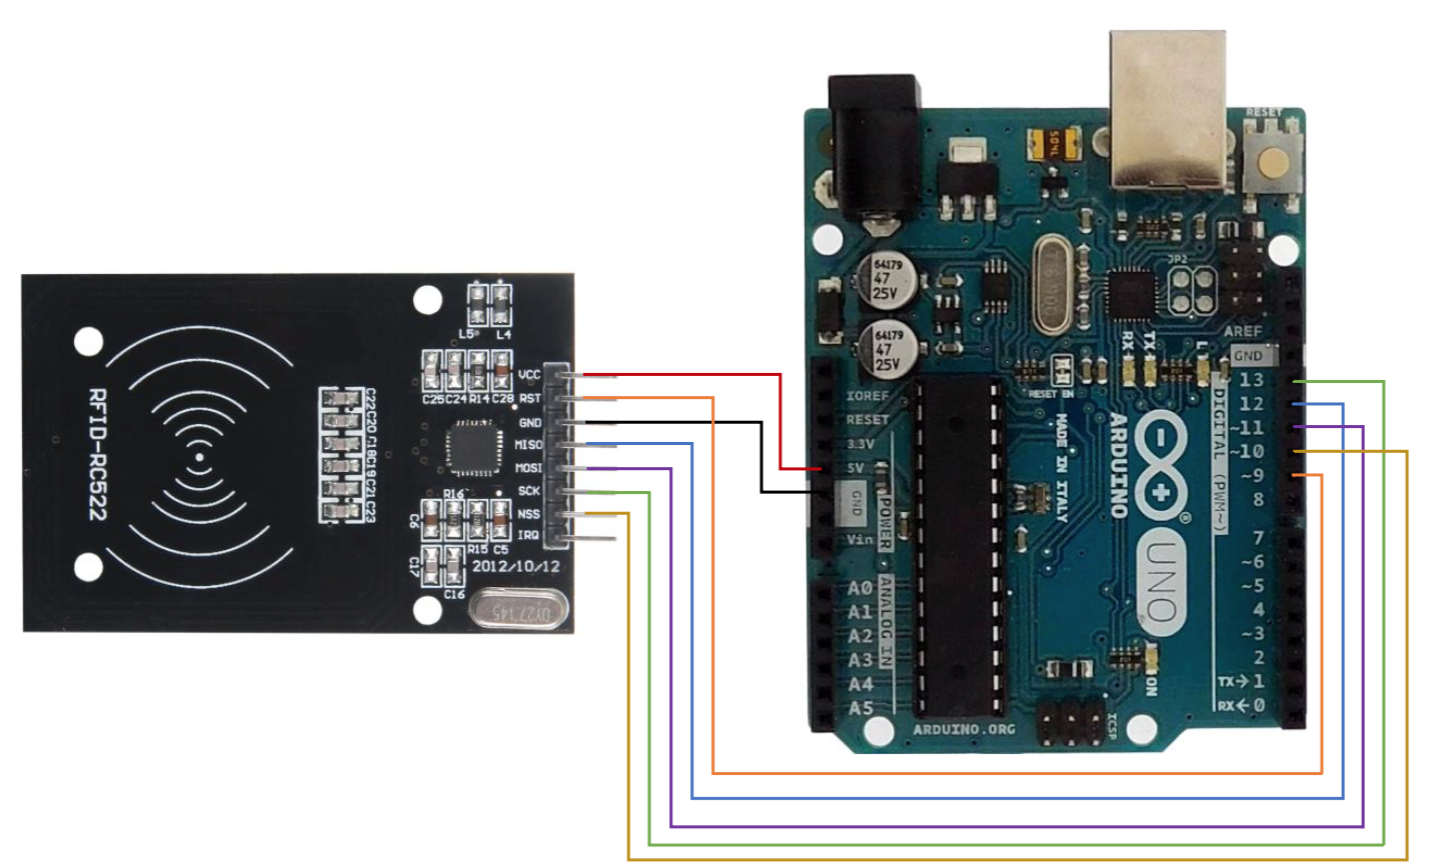
\includegraphics[width=\textwidth]{cablage}\\
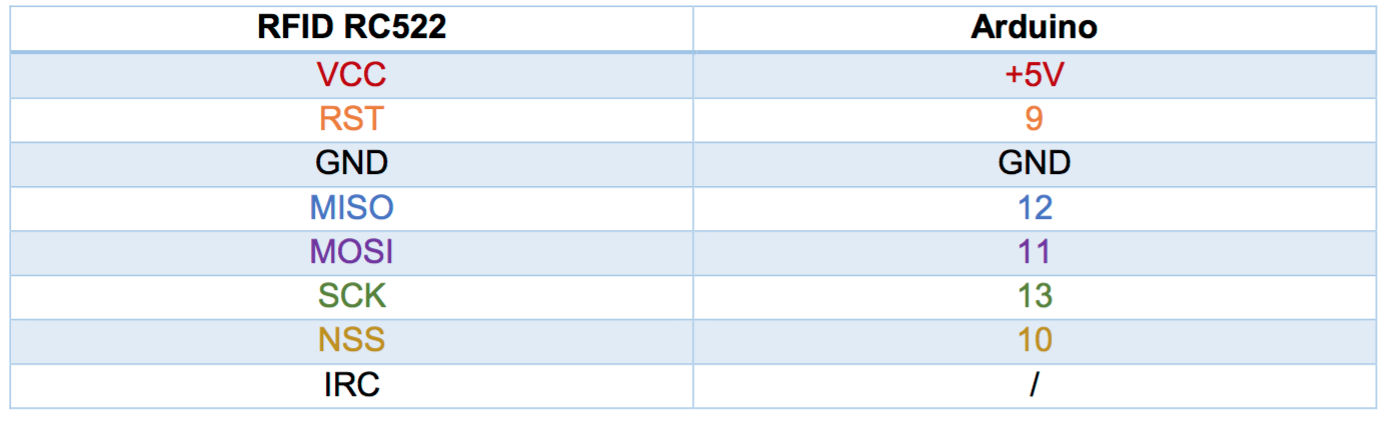
\includegraphics[width=\textwidth]{pinout}
\caption{Connection du lecteur RFID à la carte arduino}
\end{center}
\end{figure}

\question Quel est le bus qui relie le arduino et le lecteur de tag RFID ?
\reponse

\question Decrire le role de chaque fil ?
\reponse
\reponse
\reponse



\question Implémentez le code suivant : \footnote{http://makecourse.weebly.com/week10segment1.html}


\begin{lstlisting}
/*
 * MFRC522 - Library to use ARDUINO RFID MODULE KIT 13.56 MHZ WITH TAGS SPI W AND R BY COOQROBOT.
 * The library file MFRC522.h has a wealth of useful info. Please read it.
 * The functions are documented in MFRC522.cpp.
 *
 * Based on code Dr.Leong   ( WWW.B2CQSHOP.COM )
 * Created by Miguel Balboa (circuitito.com), Jan, 2012.
 * Rewritten by Soren Thing Andersen (access.thing.dk), fall of 2013
 * (Translation to English, refactored, comments, anti collision, cascade levels.)
 * Released into the public domain.
 *
 * Sample program showing how to read data from a PICC using a MFRC522 reader on the Arduino SPI interface.
 *----------------------------------------------------------------------------- empty_skull
 * Aggiunti pin per arduino Mega
 * add pin configuration for arduino mega
 * http://mac86project.altervista.org/
 ----------------------------------------------------------------------------- Nicola Coppola
 * Pin layout should be as follows:
 * Signal     Pin              Pin               Pin
 *            Arduino Uno      Arduino Mega      MFRC522 board
 * ------------------------------------------------------------
 * Reset      9                5                 RST
 * SPI SS     10               53                SDA
 * SPI MOSI   11               52                MOSI
 * SPI MISO   12               51                MISO
 * SPI SCK    13               50                SCK
 *
 * The reader can be found on eBay for around 5 dollars. Search for "mf-rc522" on ebay.com.
 */

#include <SPI.h>
#include <MFRC522.h>

#define SS_PIN 10
#define RST_PIN 9
MFRC522 mfrc522(SS_PIN, RST_PIN);	// Create MFRC522 instance.

void setup() {
  Serial.begin(9600);	// Initialize serial communications with the PC
  SPI.begin();			// Init SPI bus
  mfrc522.PCD_Init();	// Init MFRC522 card
  Serial.println("Scan PICC to see UID and type...");
}

void loop() {
  // Look for new cards
  if ( ! mfrc522.PICC_IsNewCardPresent()) {
    return;//go to start of loop if there is no card present
  }
  // Select one of the cards
  if ( ! mfrc522.PICC_ReadCardSerial()) {
    //if ReadCardSerial returns 1,
    // the "uid" struct (see MFRC522.h lines 238-45)) contains the ID of the read card.
    return;
  }
  // Dump debug info about the card. PICC_HaltA() is automatically called.
  mfrc522.PICC_DumpToSerial(&(mfrc522.uid));
}
\end{lstlisting}



\question Lecture de la carte

\tcbox{\textbf{Constatation professeur :} \hspace{5cm} } % package tcolorbox

%}}}

\partie{Lire le tag}\\ %{{{1

\question Ecrire le tag avec des données de votre choix
\begin{lstlisting}

/******************************************
        PURPOSE:	Learn to use the MF522-AN RFID card reader
	Created by      Rudy Schlaf for www.makecourse.com
	DATE:		2/2014
*******************************************/

/*
 * This sketch uses the MFRC522 Library to use ARDUINO RFID MODULE KIT 13.56 MHZ WITH TAGS SPI W
 * AND R BY COOQROBOT.
 * The library file MFRC522.h has a wealth of useful info. Please read it.
 * The functions are documented in MFRC522.cpp.
 *
 * Based on code Dr.Leong   ( WWW.B2CQSHOP.COM )
 * Created by Miguel Balboa (circuitito.com), Jan, 2012.
 * Rewritten by Soren Thing Andersen (access.thing.dk), fall of 2013 (Translation to English,
 * refactored, comments, anti collision, cascade levels.)
 *
 * This library has been released into the public domain.
*/


#include <SPI.h>//include the SPI bus library
#include <MFRC522.h>//include the RFID reader library

#define SS_PIN 10  //slave select pin
#define RST_PIN 5  //reset pin
MFRC522 mfrc522(SS_PIN, RST_PIN);        // instatiate a MFRC522 reader object.
MFRC522::MIFARE_Key key;//create a MIFARE_Key struct named 'key', which will hold the card information


void setup() {
        Serial.begin(9600);        // Initialize serial communications with the PC
        SPI.begin();               // Init SPI bus
        mfrc522.PCD_Init();        // Init MFRC522 card (in case you wonder what PCD means: proximity
				   // coupling device)
        Serial.println("Scan a MIFARE Classic card");

        // Prepare the security key for the read and write functions - all six key bytes are set to
	//   0xFF at chip delivery from the factory.
        // Since the cards in the kit are new and the keys were never defined, they are 0xFF
        // if we had a card that was programmed by someone else, we would need to know the key to
	//   be able to access it. This key would then need to be stored in 'key' instead.

        for (byte i = 0; i < 6; i++) {
                key.keyByte[i] = 0xFF;//keyByte is defined in the "MIFARE_Key" 'struct' definition in the
		                      //  .h file of the library
        }

}

int block=2; //this is the block number we will write into and then read. Do not write
	     //  into 'sector trailer' block, since this can make the block unusable.

//an array with 16 bytes to be written into one of the 64 card blocks is defined
byte blockcontent[16] = {"makecourse_____"};
//byte blockcontent[16] = {0,0,0,0,0,0,0,0,0,0,0,0,0,0,0,0};//all zeros.
//This can be used to delete a block.
//This array is used for reading out a block. The MIFARE_Read method
//requires a buffer that is at least 18 bytes to hold the 16 bytes of a block.
byte readbackblock[18];

void loop()
{

  /*********************************establishing contact with a tag/card**************************************************************/

  // Look for new cards (in case you wonder what PICC means: proximity integrated circuit card)
  if ( ! mfrc522.PICC_IsNewCardPresent()) {//if PICC_IsNewCardPresent returns 1, a new card has been found and we continue
    return;//if it did not find a new card is returns a '0' and we return to the start of the loop
  }

  // Select one of the cards
  //if PICC_ReadCardSerial returns 1, the "uid" struct (see MFRC522.h lines 238-45)) contains the ID of the read card.
  if ( ! mfrc522.PICC_ReadCardSerial()) {
    //if it returns a '0' something went wrong and we return to the start of the loop
    return;
  }

  // Among other things, the PICC_ReadCardSerial() method reads the UID and the SAK (Select acknowledge) into the mfrc522.uid struct,
  //   which is also instantiated during this process.
  // The UID is needed during the authentication process
  //The Uid struct:
  //typedef struct {
  //byte		size;			// Number of bytes in the UID. 4, 7 or 10.
  //byte		uidByte[10];            //the user ID in 10 bytes.
  //byte		sak;			// The SAK (Select acknowledge) byte returned from the PICC after successful selection.
  //} Uid;

  Serial.println("card selected");

  /*********************************writing and reading a block on the card**************************************************************/

  writeBlock(block, blockcontent);//the blockcontent array is written into the card block
  //mfrc522.PICC_DumpToSerial(&(mfrc522.uid));

  //The 'PICC_DumpToSerial' method 'dumps' the entire MIFARE data block into the serial monitor.
  \\Very useful while programming a sketch with the RFID reader...
  //Notes:
  //(1) MIFARE cards conceal key A in all trailer blocks, and shows 0x00 instead of 0xFF.
  //    This is a secutiry feature. Key B appears to be public by default.
  //(2) The card needs to be on the reader for the entire duration of the dump.
  //    If it is removed prematurely, the dump interrupts and an error message will appear.
  //(3) The dump takes longer than the time alloted for interaction per pairing between reader and card,
  //    i.e. the readBlock function below will produce a timeout if the dump is used.

  //mfrc522.PICC_DumpToSerial(&(mfrc522.uid));//uncomment this if you want to see the entire 1k memory with the block written into it.

  readBlock(block, readbackblock);//read the block back
  Serial.print("read block: ");
  for (int j=0 ; j<16 ; j++)//print the block contents
  {
    Serial.write (readbackblock[j]);//Serial.write() transmits the ASCII numbers as human readable characters to serial monitor
  }
  Serial.println("");
 }

\end{lstlisting}

%}}}
\tcbox{\textbf{Constatation professeur :} \hspace{5cm} } % package tcolorbox


\end{document}
%vim:fdm=marker

